\chapter{Execução à nível de Portfólio}
  
  Esse capítulo apresenta as atividades e resultados obtidos na execução do processo a nível de Portfólio.
  
  \begin{figure}[!htbp]
    \centering
    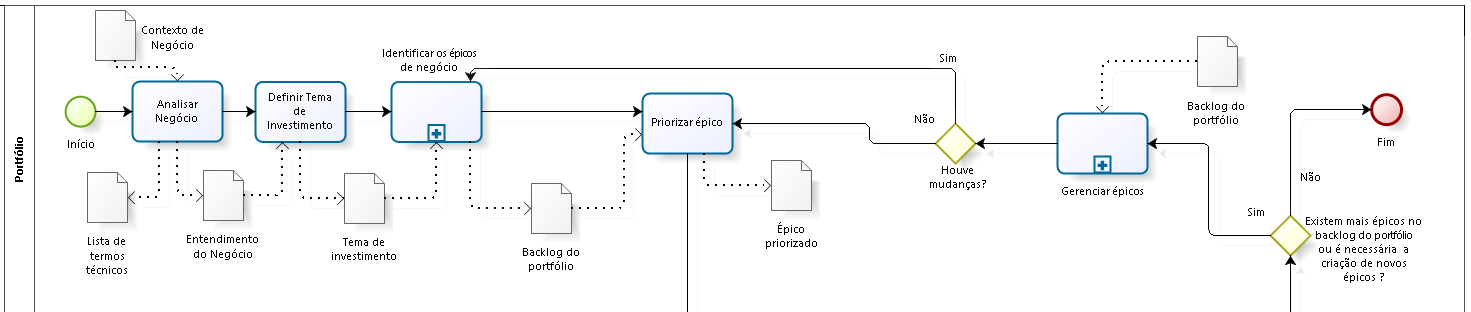
\includegraphics[scale=0.33]{figuras/processo_portfolio}
    \caption[Processo - Nível de Portfólio]{Processo - Nível de Portfólio.}
    \label{processo_portfolio}
  \end{figure}
   
  \section{Reuniões realizadas}
    
    Foram realizadas três reuniões entre a equipe de requisitos e o cliente, no contexto do nível de Portfólio.
    Esta seção apresenta um breve resumo das reuniões.
    
    \subsection{Resumo da 1ª reunião}
      
      Primeiramente, a equipe de requisitos analisou o contexto de negócio que foi proposto.
      Com a análise do contexto de negócio proposto, foi realizada a primeira reunião com o cliente, que tinha o objetivo de 
      obter um entendimento inicial do negócio por parte da equipe de requisitos. 
      
      Para obter o entendimento do negócio, a equipe de requisitos levantou perguntas com base no contexto de negócio apresentado, 
      de modo que as perguntas guiassem o rumo da entrevista.
      
      O objetivo da reunião foi atingido com o entendimento do negócio estabelecido entre as partes. Nessa reunião 
      foram levantados também alguns termos técnicos para o contexto da organização, que se encontram no documento de visão
      (em apêndice).
      
    \subsection{Resumo da 2ª reunião}
    
      Com o entendimento de negócio estabelecido, a equipe de requisitos analisou os processos e atividades da 
      organização para definir o problema da organização. A segunda reunião foi realizada para a validação do problema 
      da organização junto ao cliente.
      
      Nessa reunião ainda foi possível definir o Tema de Investimento da organização.
    
    \subsection{Resumo da 3ª reunião}
    
      Com o Tema de Investimento validado, a equipe de requisitos identificou possíveis épicos de negócio e foi realizada a terceira
      reunião utilizando a técnica de entrevista para o levantamento e validação dos épicos junto ao cliente.
      
      A equipe de requisitos criou perguntas para obter respostas do cliente que permitissem a avaliação dos épicos identificados.
      Nessa reunião também foi possível levantar algumas características do sistema.
    
  \section{Entendimento do negócio}
  
      Com o aumento do número de viaturas (caminhões, ônibus, ambulâncias, carros, motos, barcos e helicópteros) do Corpo de 
  Bombeiros Militar do Distrito Federal (CBMDF), houve a necessidade de gerenciar com maior rigor e precisão.

  \begin{figure}[!htbp]
    \centering
    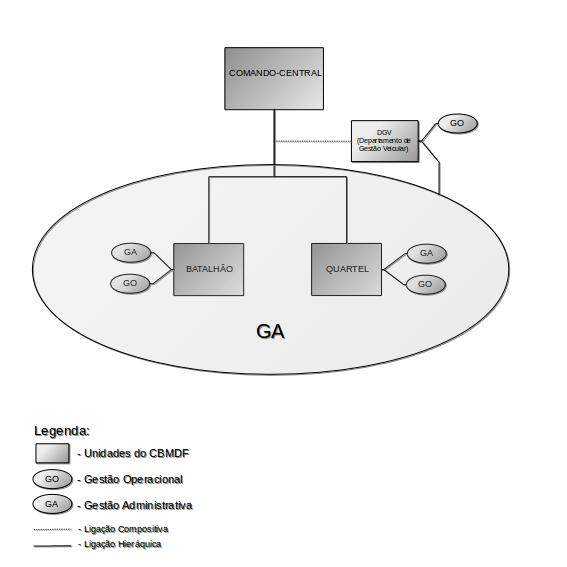
\includegraphics[scale=0.7, angle=0]{figuras/entendimento_negocio}
    \caption{Organograma do CBMDF para o contexto de negócio.}
    \label{entendimento_negocio}
  \end{figure}
  
  A Figura \ref{entendimento_negocio} acima representa, organizacionalmente, as unidades do Corpo de Bombeiros Militar do Distrito Federal (CBMDF)
  envolvidas no contexto de negócio proposto para este projeto. As unidades estão dispostas hierarquicamente. 
  O Comando-Central é a unidade de maior escalão do CBMDF e, atualmente, possui grande dificuldade em obter uma ampla 
  visão das informações acerca de suas viaturas.
  
  O Departamento de Gestão Veicular (DGV) é a partição dentro do Comando-Central responsável pelo gerenciamento de todas 
  as viaturas da Corporação, incumbida da Gestão Administrativa de todo o CBMDF, no que diz respeito ao gerenciamento das 
  viaturas. Já as demais unidades (Batalhões e Quarteis) possuem a responsabilidade de gerenciar suas viaturas, de forma 
  independente, realizando as Gestões Administrativa e Operacional das viaturas inerentes à sua unidade.
  
  Cada unidade realiza as atividades das gestões administrativa e operacional independentemente e de forma despadronizada, 
  além de que todos os registros são feitos em planilhas eletrônicas, onde cada unidade possui suas próprias planilhas, 
  caracterizando uma descentralização das informações. Essa descentralização, falta das informações em tempo real, engessa 
  a comunicação entre as unidades e o DGV, este que tem que solicitar as informações para as unidades, juntá-las e interpretar 
  os dados para realizar a gestão administrativa das viaturas de toda a corporação.
  
  A gestão administrativa compreende as atividades de controle do custo do combustível, alocação das viaturas nas unidades
  (pelo DGV), acompanhamento da situação das viaturas e a gestão dos motoristas das unidades.
  
  A gestão operacional compreende as atividades no âmbito das operações realizadas pelas unidades, como o gerenciamento das 
  missões de uma unidade, vinculação de viaturas às missões, controle do consumo de combustível e verificação de 
  disponibilidade de viaturas.
  
  \vfill
  \pagebreak
    
  \section{Problema da organização}
    
    
  \textbf{O problema:} Ineficiência da gestão das informações acerca das viaturas.
  
  \textbf{Afeta:} Corpo de Bombeiros e população do DF.
  
  \textbf{Cujo impacto é:} Tomadas de decisões inadequadas, falta de qualidade de vida para os bombeiros e gastos desnecessários.
  
  \textbf{Uma solução bem sucedida seria:} Um sistema que centralizaria as informações acerca das viaturas, as fornecendo 
  em tempo real para quem necessitasse das mesmas.
  
  \section{Considerações finais a nível de Portfólio}
    
    Esta seção apresenta um resumo dos itens mais importantes produzidos a nível de Portfólio.
    
    \subsection{Tema de investimento definido}
      
      O seguinte tema de investimento ficou definido para a organização:
      
      \emph{Tema de investimento (T1): Gestão de viaturas.}
    
    \subsection{Épicos identificados}
      
      O \textit{Backlog} do Portfólio ficou composto pelos seguintes épicos:
      
      \begin{itemize}
      \item \emph{Épico 1 (T1E1) – Gestão Operacional nas unidades;}
      \item \emph{Épico 2 (T1E2) – Gestão Administrativa nas unidades.}
      \end{itemize}

    